\documentclass[a4paper, 12pt]{article}
\usepackage{cmap}
\usepackage{amssymb}
\usepackage{amsmath}
\usepackage{graphicx}
\usepackage{amsthm}
\usepackage{upgreek}
\usepackage{setspace}
\usepackage{color}
\usepackage{pgfplots}
\pgfplotsset{compat=1.9}
\usepackage[T2A]{fontenc}
\usepackage[utf8]{inputenc}
\usepackage[normalem]{ulem}
\usepackage{mathtext} % русские буквы в формулах
\usepackage[left=2cm,right=2cm, top=2cm,bottom=2cm,bindingoffset=0cm]{geometry}
\usepackage[english,russian]{babel}
\usepackage[unicode]{hyperref}
\newenvironment{Proof} % имя окружения
{\par\noindent{$\blacklozenge$}} % команды для \begin
{\hfill$\scriptstyle\boxtimes$}
\newcommand{\Rm}{\mathbb{R}}
\newcommand{\Cm}{\mathbb{C}}
\newcommand{\Z}{\mathbb{Z}}
\newcommand{\I}{\mathbb{I}}
\newcommand{\N}{\mathbb{N}}
\newcommand{\rank}{\operatorname{rank}}
\newcommand{\Ra}{\Rightarrow}
\newcommand{\ra}{\rightarrow}
\newcommand{\FI}{\Phi}
\newcommand{\Sp}{\text{Sp}}
\renewcommand{\leq}{\leqslant}
\renewcommand{\geq}{\geqslant}
\renewcommand{\alpha}{\upalpha}
\renewcommand{\beta}{\upbeta}
\renewcommand{\gamma}{\upgamma}
\renewcommand{\delta}{\updelta}
\renewcommand{\varphi}{\upvarphi}
\renewcommand{\phi}{\upvarphi}
\renewcommand{\tau}{\uptau}
\renewcommand{\lambda}{\uplambda}
\renewcommand{\psi}{\uppsi}
\renewcommand{\mu}{\upmu}
\renewcommand{\omega}{\upomega}
\renewcommand{\d}{\partial}
\renewcommand{\xi}{\upxi}
\renewcommand{\epsilon}{\upvarepsilon}
\newcommand{\intx}{\int\limits_{x_0}^x}
\newcommand\Norm[1]{\left\| #1 \right\|}
\newcommand{\sumk}{\sum\limits_{k=0}^\infty}
\newcommand{\sumi}{\sum\limits_{i=0}^\infty}
\newtheorem*{theorem}{Теорема}
\newtheorem*{cor}{Следствие}
\newtheorem*{lem}{Лемма}
\begin{document}
	\section*{Интерполяционный многочлен с кратными узлами}
	\subsubsection*{Условие}
	Построить интерполяционный многочлен для функции $f(x) = x^6$ по следующей таблице входных данных: $f(0), f'(0), f''(0), f(1), f'(1)$. Вычислить с его помощью приближенное значение $f(0.5)$ и оценить погрешность найденного значения.
	\subsubsection*{Алгоритм решения}
	Для решения данной задачи потребуются следующие формулы:
	\begin{enumerate}
		\item остаток интерполирования при интерполировании с кратными узлами 
		\begin{eqnarray}
			r_n(x) = \Omega(x) \dfrac{f^{(n+1)}(\xi)}{(n+1)!},\quad \Omega (x) = (x-x_0)^{\alpha_0}\ldots (x-x_m)^{\alpha_m},\ \xi \in [a,b].
		\end{eqnarray}
		\item представление многочлена Эрмита через разделенные разности
		\begin{multline}
			P_n(x) = f(x_0) + (x-x_0)f(x_0, x_0) + \ldots + (x-x_0)^{\alpha_0-1}f(x_0,\ldots, x_0) + \\ + (x-x_0)^{\alpha_0}f(x_0,\ldots, x_0; x_1)+ (x-x_0)^{\alpha_0}(x-x_1)f(x_0,\ldots, x_0; x_1, x_1) +\ldots +\\+ \ldots + (x-x_0)^{\alpha_0}(x-x_1)^{\alpha_1-1} f(x_0,\ldots, x_0; x_1,\ldots, x_1) + \ldots+ \\\ +\ldots + (x-x_0)^{\alpha_0}(x-x_1)^{\alpha_1}\ldots(x-x_m)^{\alpha-1}f(x_0,\ldots x_0; x_1,\ldots, x_1; \ldots; x_{m},\ldots, x_{m}).
		\end{multline}
		\item для построения таблицы разделенных разностей, необходимо учитывать соотношение 
		\begin{eqnarray}
			f(\underbrace{x_0,\ldots, x_0}_{j+1}) = \dfrac{f^{(j)}(x_0)}{j!}
		\end{eqnarray}
		\item аппарат разделенных разностей:
		\begin{itemize}
			\item \textbf{разделенная разность нулевого порядка для функции $f(x)$} совпадают со значениями функции $f(x_i)$ в узлах интерполирования;
			\item \textbf{разделенная разность первого порядка} есть \begin{eqnarray}
				f(x_i, x_j) = \dfrac{f(x_j) - f(x_i)}{x_j - x_i}.
			\end{eqnarray}
			\item \textbf{разделенная разность второго порядка} \begin{eqnarray}
				f(x_i, x_j, x_k) = \dfrac{f(x_j, x_k) - f(x_i, x_j)}{x_k - x_i}.
			\end{eqnarray}
			\item \textbf{разделенная разность $(k+1)$-ого порядка} \begin{eqnarray}
				f(x_0, \ldots, x_{k+1}) = \dfrac{f(x_1,\ldots, x_{k+1}) - f(x_0,\ldots, x_k)}{x_{k+1} - x_0}.
			\end{eqnarray}
		\end{itemize}
		\item таблица разделенных разностей
		$$
		\includegraphics[scale=0.35]{"C:/Users/bzzdwn/Documents/Конспекты/Computational Methods/img9"}
		$$
	\end{enumerate}
	Алгоритм решения задачи следующий: составляем таблицу разделенных разностей, записываем интерполяционный многочлен, вычисляем значение в нужной точке, оцениваем остаток интерполирования в этой точке.\\\\
	Для начала рассчитаем входные данные:
	$$f(0) = 0,\quad f'(0) = 0,\quad f''(0) = 0,\quad f(1) = 1,\quad f'(1) = 6.$$
	Далее составляем таблицу конечных разностей, которая в нашем случае примет вид 
	$$
		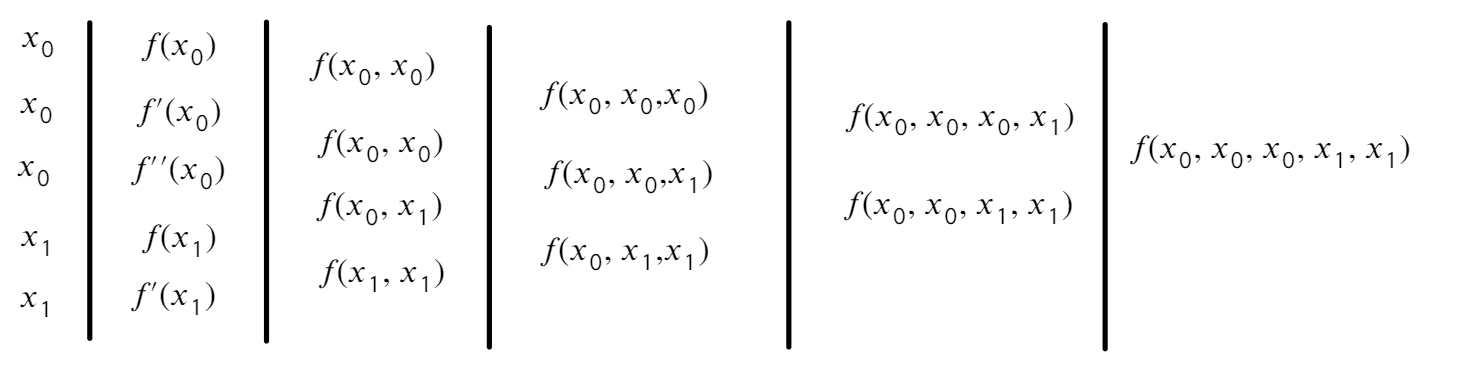
\includegraphics[scale=0.45]{img7}
	$$
	Заполним первые два столбца известными нам значениями:
	$$
		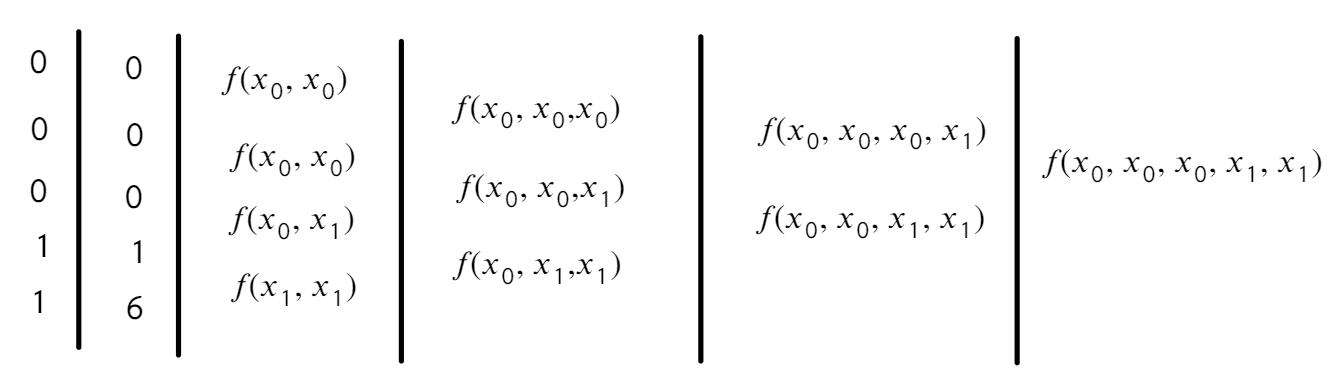
\includegraphics[scale=0.45]{img8}
	$$
	По формуле (3) $$f(x_0, x_0) = \dfrac{f'(x_0)}{1!} = 0,\quad f(x_1, x_1) = \dfrac{f'(x_1)}{1!} = 6.$$
	По формуле (4) $$f(x_0, x_1) = \dfrac{f(x_1) - f(x_0)}{x_1 - x_0} = 1.$$
	$$
		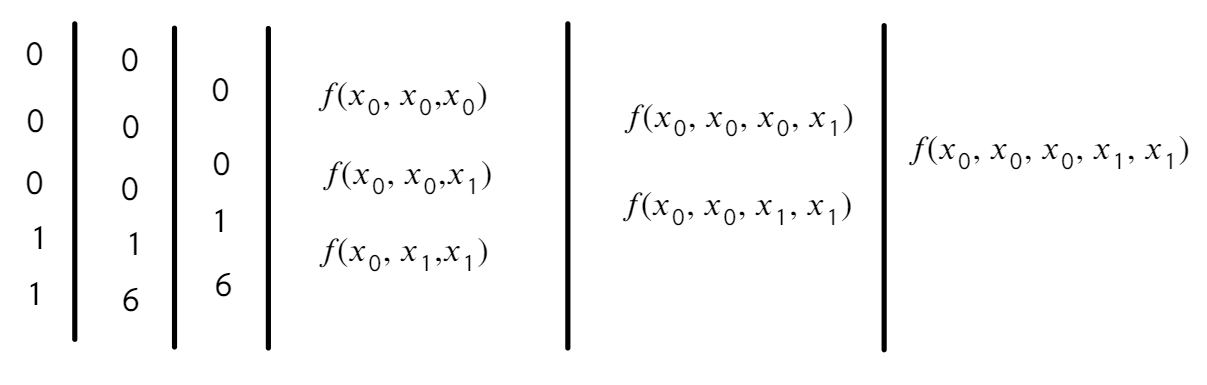
\includegraphics[scale=0.45]{img9}
	$$
	По формуле (3) $$f(x_0, x_0, x_0) = \dfrac{f'(x_0)}{2!} = 0.$$
	По формуле (5) $$f(x_0, x_0, x_1) = \dfrac{f(x_0,x_1) - f(x_0, x_0)}{x_1 - x_0} = 1,\quad f(x_0, x_1, x_1) = \dfrac{f(x_1,x_1) - f(x_0, x_1)}{x_1 - x_0} = 5.$$
	Далее аналогично по формуле (6)
	$$f(x_0, x_0, x_0, x_1) = \dfrac{f(x_0, x_0, x_1) - f(x_0, x_0, x_0)}{x_1 - x_0} = 1,\quad f(x_0, x_0, x_1, x_1) = \dfrac{f(x_0, x_1, x_1) - f(x_0, x_0, x_1)}{x_1 - x_0} = 4.$$
	И в итоге $$f(x_0,x_0,x_0,x_1,x_1) = \dfrac{f(x_0, x_0, x_1, x_1) -f(x_0, x_0, x_0, x_1) }{x_1 - x_0} = 3.$$
	Тогда таблица принимает окончательный вид
	$$
		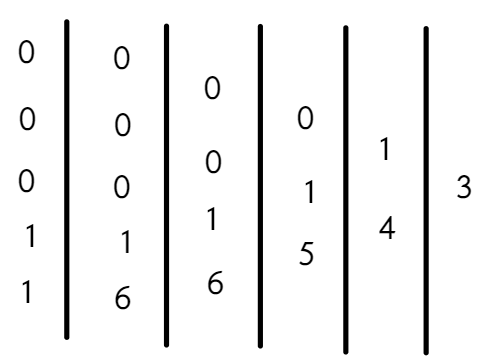
\includegraphics[scale=0.45]{img10}
	$$
	Из этой таблицы нам нужны лишь значения
	$$
		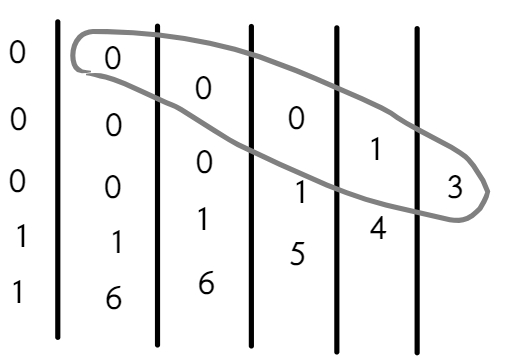
\includegraphics[scale=0.45]{img11}
	$$
	Далее по формуле (2) запишем сначала интерполяционный многочлен в общем виде для нашего случая (5 узлов $\Rightarrow$ 4 степень многочлена)
	\begin{multline*}
		P_4(x) = f(x_0) + (x-x_0)f(x_0, x_0) + (x-x_0)^2f(x_0, x_0,x_0)+\\+ (x-x_0)^3f(x_0, x_0,x_0, x_1) + (x-x_0)^3(x-x_1)f(x_0, x_0,x_0, x_1, x_1).
	\end{multline*}
	Подставляем все известные нам значения и получаем
	$$P_4(x) = 0 + x\cdot 0 + x^2\cdot 0 + x^3\cdot 1 + x^3(x_1)\cdot 3 = 3x^4 - 2x^3.$$
	Можно, подставив известные точки и их значения, убедиться в том, что многочлен был построен правильно. \\\\
	Вычислим значение в точке $x=0.5$:
	$$P_4(0.5) = \dfrac{3}{16} - \dfrac{2}{8} = -\dfrac{1}{16}.$$
	Оценим остаток по формуле (1). Для начала запишем его в общем виде для нашего случая:
	$$r_4(x) = (x-x_0)^3 ( x-x_1)^2\cdot \dfrac{f^{(5)}(\xi)}{5!},\quad \xi \in [0,1].$$
	Нам неизвестно значение $f^{(5)}(\xi)$. Оценим его сверху:
	$$f^{(5)}(x) = (x^6)^{(5)} = 720 x\Rightarrow |f^{(5)}(x)| \leq 720 \quad x\in [0,1].$$
	Тогда оценка для остатка примет вид
	$$|r_4(x)|\leq \left|x^3 ( x-1)^2\cdot \dfrac{720}{120}\right| = 6\left|x^3 ( x-1)^2\right|.$$
	Отсюда погрешность вычисленного значения в точке $x=0.5$ составляет $$|r_4(0.5)|\leq 6\left|\dfrac{1}{2^3} \cdot\dfrac{1}{2^2}\right| = \dfrac{3}{16}.$$
\end{document} 